\documentclass[12pt, a4paper]{scrartcl}
\usepackage[utf8]{inputenc}
\usepackage{graphicx}
\usepackage{amsmath, amsthm, amssymb, textcomp}
\usepackage{setspace}
\usepackage{paralist}
\usepackage{graphicx}
\usepackage{caption}
\graphicspath{{WSK_im/}} %Graphic is in a folder named WSK_im in the currend directory
\usepackage{float}
\usepackage{authblk}
\renewcommand\Authfont{\fontsize{12}{14.4}\selectfont}
\title{Bayesian probability theory - Lesson 2:\\
Discrete probability distributions and samples}

\author{Wolfgang von der Linden, Gerhard Dorn, Johanna Moser}
\date{Transcript}

\begin{document}
\setlength{\parindent}{0pt}
\maketitle
\onehalfspacing

Welcome to the second unit of the course on Bayesian probability theory. My name is Wolfgang von der Linden and I will enable you to help Captain Bayes and her crew to solve the questions regarding the golden nautilus wheel.
The aim of this unit is to derive probabilities from experiments, which we will call the \textbf{frequentist approach} and which in this story is represented by Captain Venn. 
The \textbf{law of large numbers} will be the central message that explains the link between intrinsic probabilities and sample estimates.
Furthermore, we extend the probabilistic language and investigate probability distributions and introduce quantities to characterize them.\\
\begin{figure}[H]
	\centering
	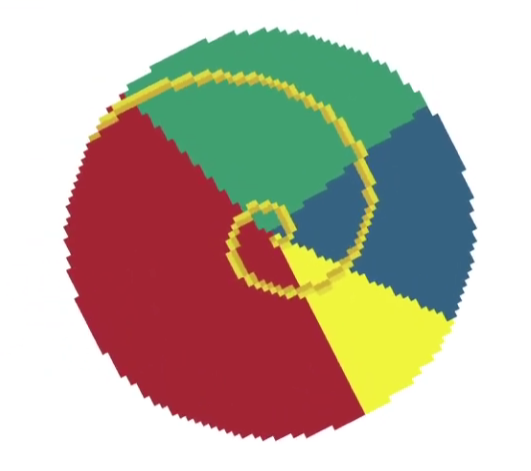
\includegraphics[width=0.45\textwidth]{2_1.png}
\end{figure}
Before we discuss probability distributions and samples, let us first review the findings of the last unit and apply them to the recent adventure of Captain Bayes: to the Golden Nautilus Wheel.
The golden Nautilus wheel has four segments for the four possible tasks of the day. These segments represent the outcomes of the random experiment and form the sample space $\Omega$.
Do you remember the concept of random variables and how we can define them? \\

\fbox{\parbox{\linewidth}{\textbf{Question 1.} How can you define a random variable?\\
a) In the case of the Nautilus wheel we can take the wages for each task (pennies).\\
b) In the case of the Nautilus wheel we can take the color as random variable.\\
c) In general you identify each outcome with a unique real number that makes it somehow meaningful.\\
d) Just take a random number.
}}\\

In principle you have to assign a number to each outcome. The number that is natural in this example is the number of pennies, which is rewarded for each task of the day. 
So, the range of the random variable in this example is $\{1,3,4,6\}$  is one three four and six. %%
Now the outcomes are represented on the abscissa and we can plot the corresponding probabilities derived by Bernoulli on the ordinate. Remember that probabilities add up to one.
The diagram, depicting probabilities over the random variable is called \textbf{``probability mass function"} and is one way to illustrate a discrete probability distribution.
\begin{figure}[H]
	\centering
	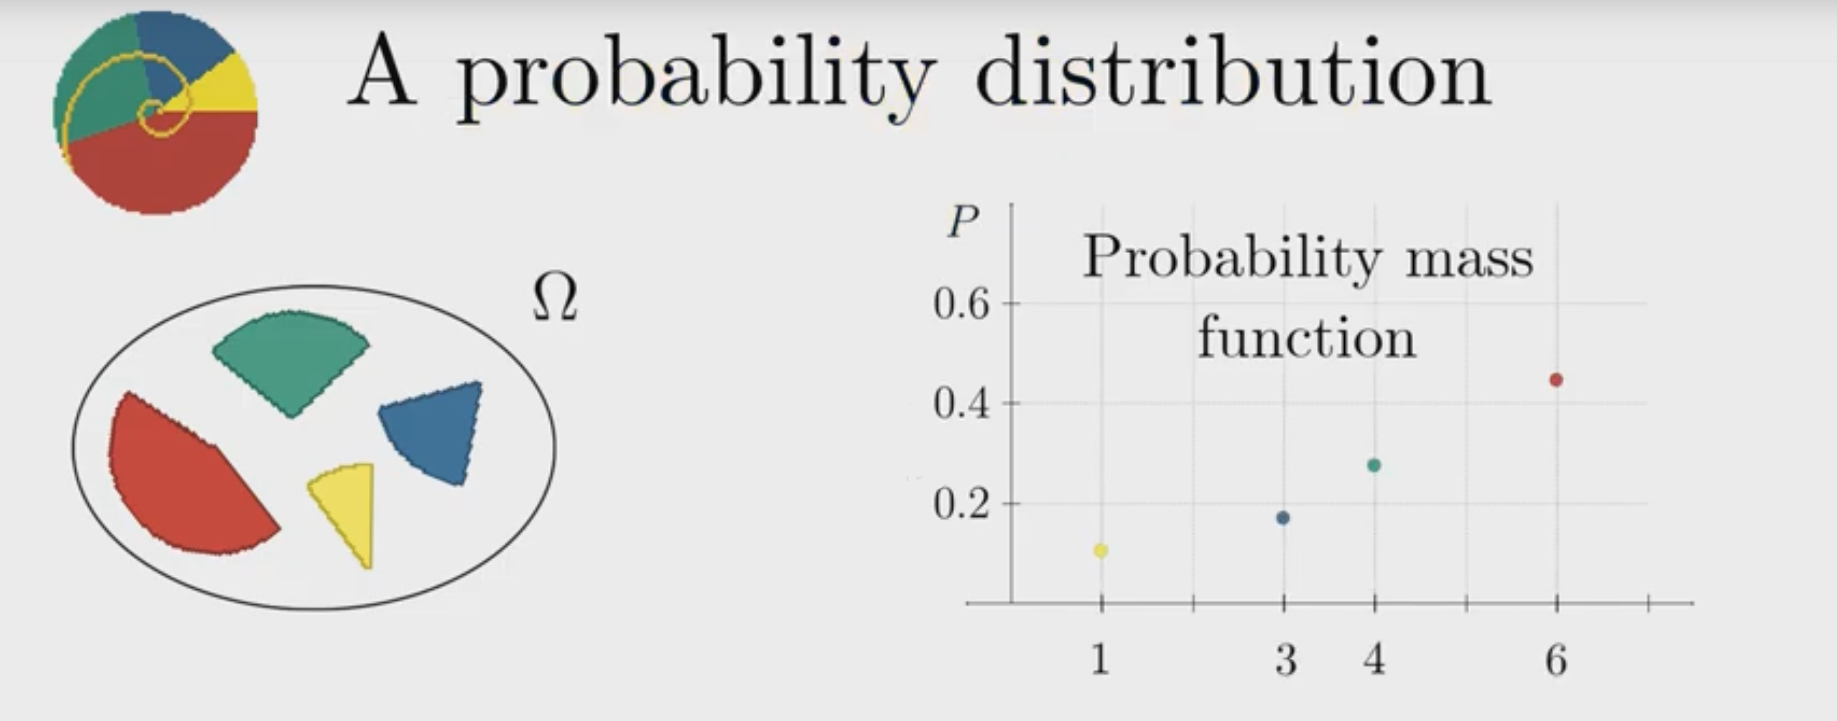
\includegraphics[width=0.75\textwidth]{2_2.png}
\end{figure}
Depending on the order in which we assign the outcomes to real numbers, we obtain different probability distributions!
To complete the review of the last unit, remember the generalization of outcomes to \textbf{events} which allows us to formulate questions like 
``What is the probability for Sailing OR Fishing".\\

\fbox{\parbox{\linewidth}{\textbf{Question 2.} What is the probability for ``Sailing'' or ``Fishing''?\\
a) $P$(Sailing)+$P$(Fishing)\\
b) $P$(Sailing)$\cdot$ $P$(Fishing)\\
c) 1- ($P$(Free Day)+$P$(Shrubbing))\\
d) $P$(Sailing) + (1 - $P$(Fishing))\\
e) $P$(Sailing) - $P$(Fishing)
}}\\

The new concept in this unit is \textbf{sampling}.
Captain Venn repeats the experiment of the golden Nautilus wheel a hundred times and collects a \textbf{sample} of the experiment, which is in principle an array of outcomes. 
A good representation of such a sample is a histogram which indicates how often an outcome occurred.
Note that different samples lead to different histograms, which can vary significantly, as can be seen in this case with sample size 24. 
\begin{figure}[H]
	\centering
	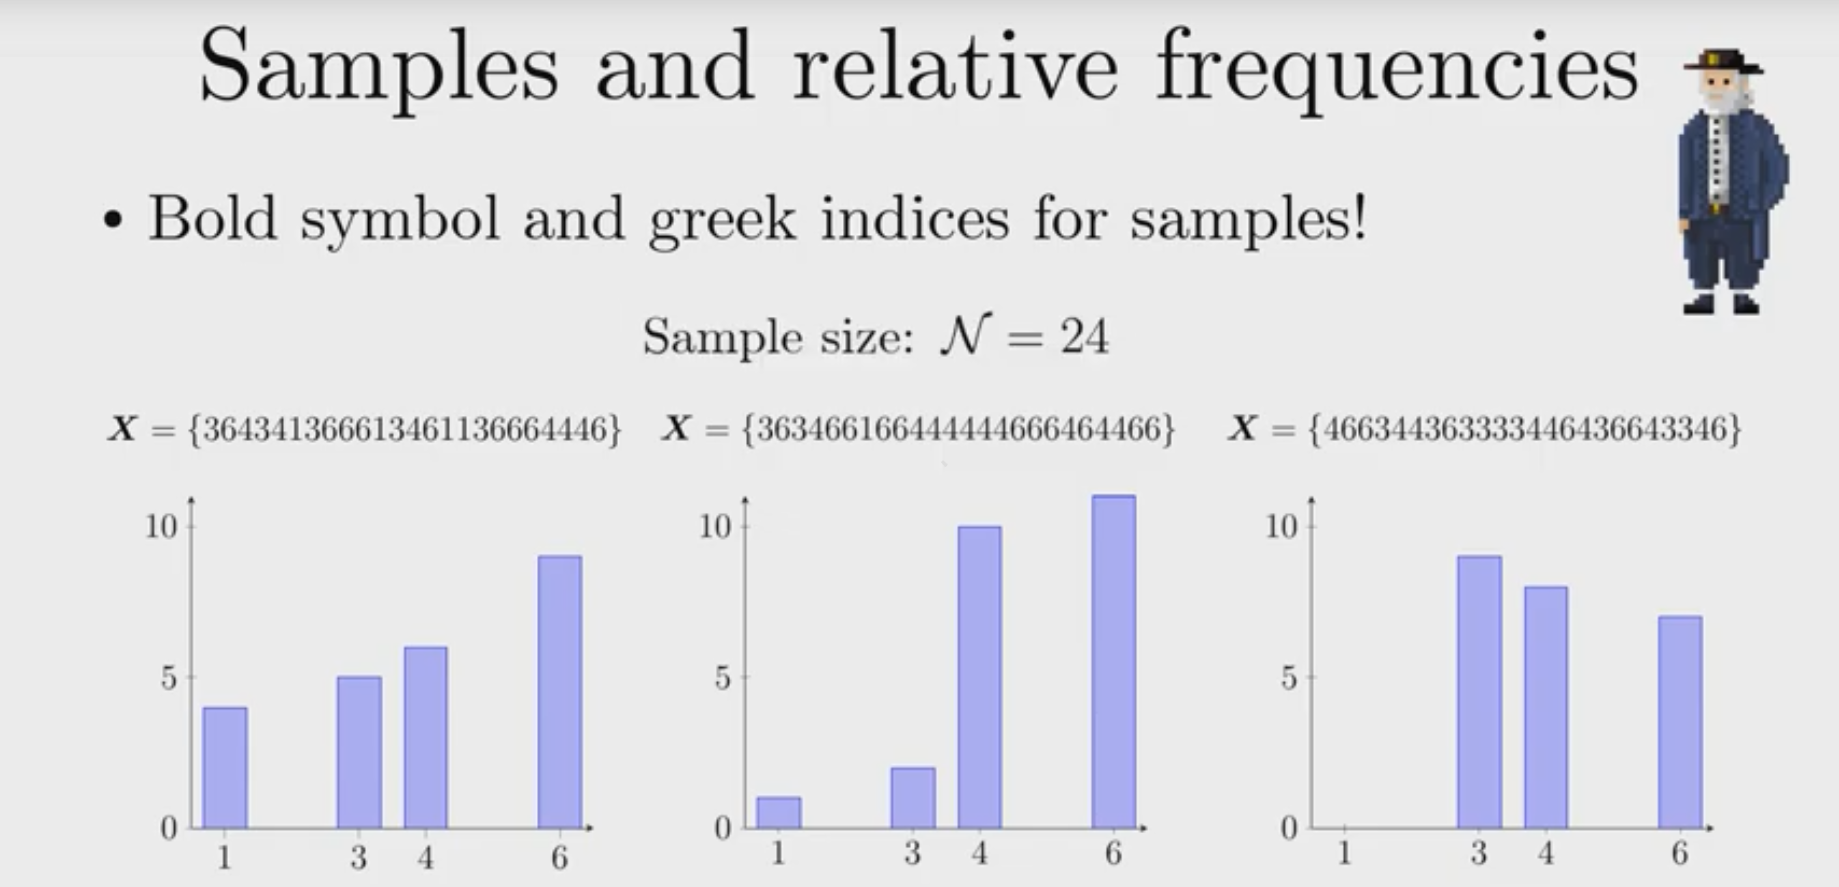
\includegraphics[width=0.75\textwidth]{2_3.png}
\end{figure}
For a large sample size, for instance 1000, the inter-sample variation is less, and the individual diagrams resemble more the intrinsic probability mass function, that we discussed before.\\

\fbox{\parbox{\linewidth}{\textbf{Question 3.} Which of the following statements is true?\\
a) We call the function that maps probabilities over the random variable $P(X)$ the probability mass function (for discrete problems).\\
b) The probabilities of the probability mass function always add up to one.\\
c) The frequencies of the outcomes of a sample are plotted in histograms.\\
d) You can directly extract the true intrinsic probabilities from histograms.\\
e) A histogram counts the probabilities of each random variable.
}}\\

This brings us to the Frequentist approach of how to define the probability of an outcome, namely by the \textit{relative frequency of its occurrence in the limit of an infinite sample size}.\\

\begin{equation*}\boxed{P_i:= \lim_{N\rightarrow \infty}\frac{N_i(X)}{N}}\end{equation*}\\
An interesting question, which will be partly answered by the \textbf{law of large numbers}, is the following: \textit{How well is the intrinsic probability approximated by the relative frequency of a finite size sample?}\\

Before discussing the law of large numbers, we enhance our language in probability theory and introduce parameters that are suited to characterize probability distributions.
The aim is to specify the form of the distribution by a few parameters that help us to make statements about the random experiment, like the average wages on Captain Venn's ship.
To be more specific, we first introduce two different distributions which we encounter again in the next units:
The \textbf{binomial distribution} that describes the probability for the number $K$ of successes in a binary experiment repeated independently $N$ times. The binomial distribution depends on two parameters: the \textbf{number of repetitions $N$} and the \textbf{success probability $Q$} in a single experiment.
Depending on these parameters, the peak centers, also called \textbf{locations}, change and so does the \textbf{width} of the peak. Note that this distribution is symmetric around its center.
\begin{figure}[H]
	\centering
	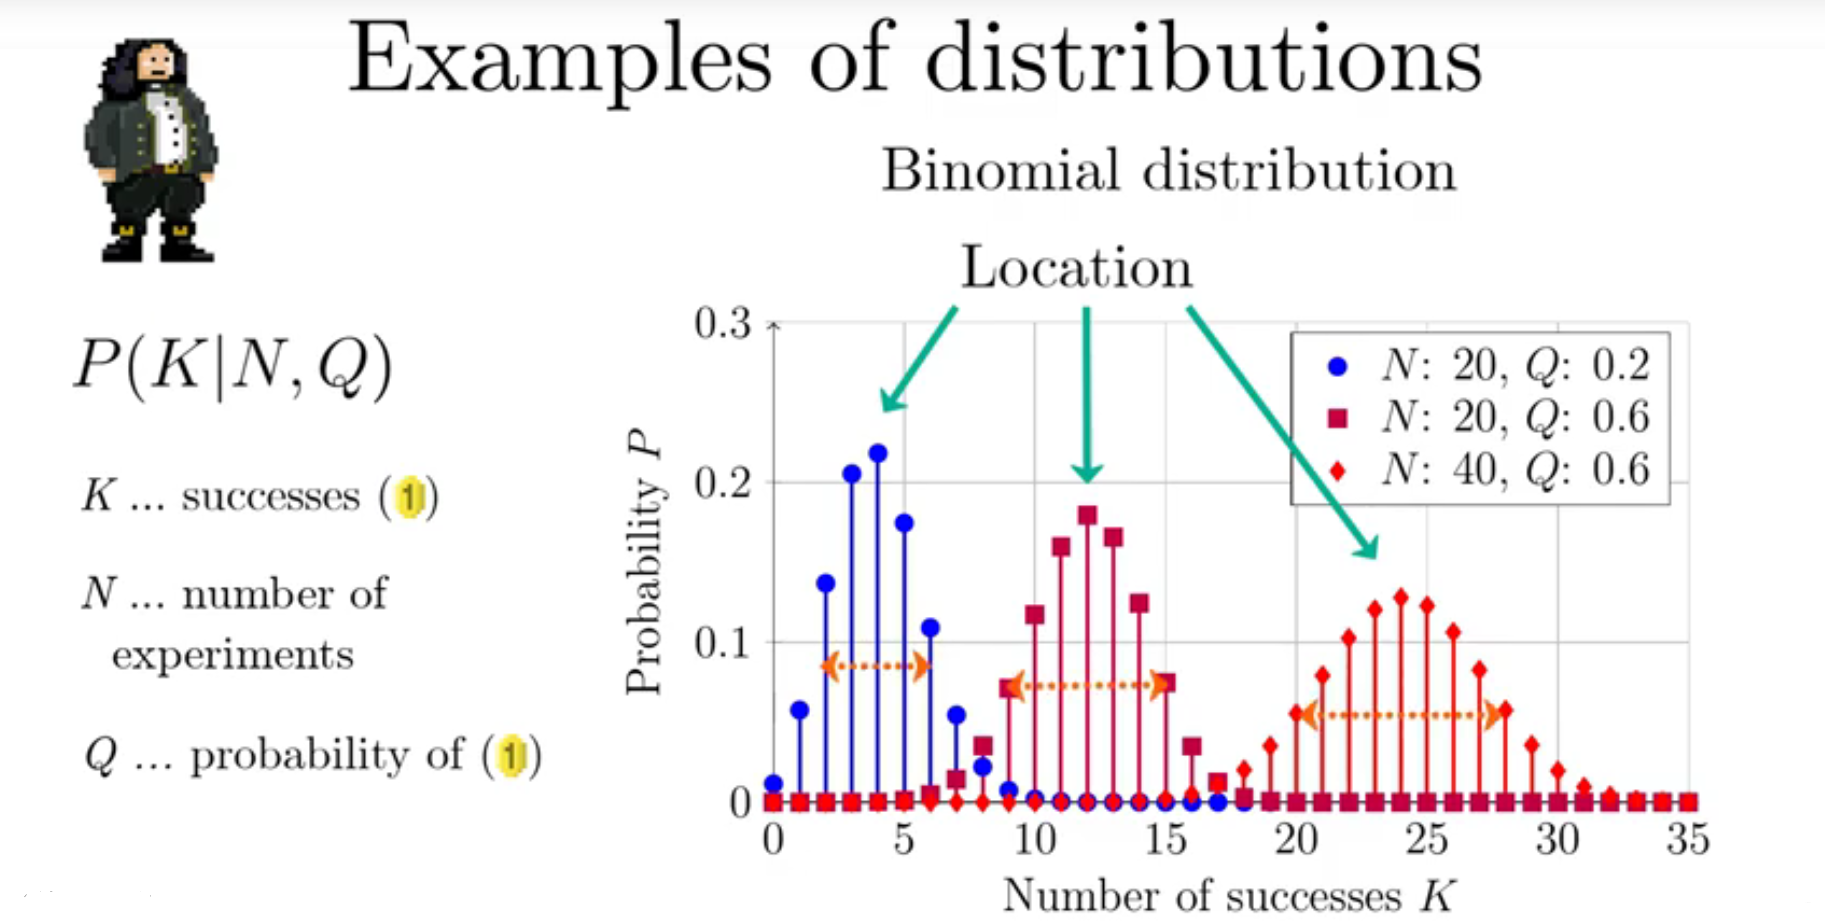
\includegraphics[width=0.75\textwidth]{2_4.png}
\end{figure}
The second example is given by the \textbf{Poisson distribution}, it provides the probability for finding \textit{k observations} of an event in a \textit{fixed time or space interval}, here the average count in that interval is known to be $\lambda$. 
The Poisson distribution occurs very often in nature, especially in the context of \textit{counting experiments}, like the number of meteorites striking the earth in a year or the number of photons emitted by a bulb per second.\\
\begin{figure}[H]
	\centering
	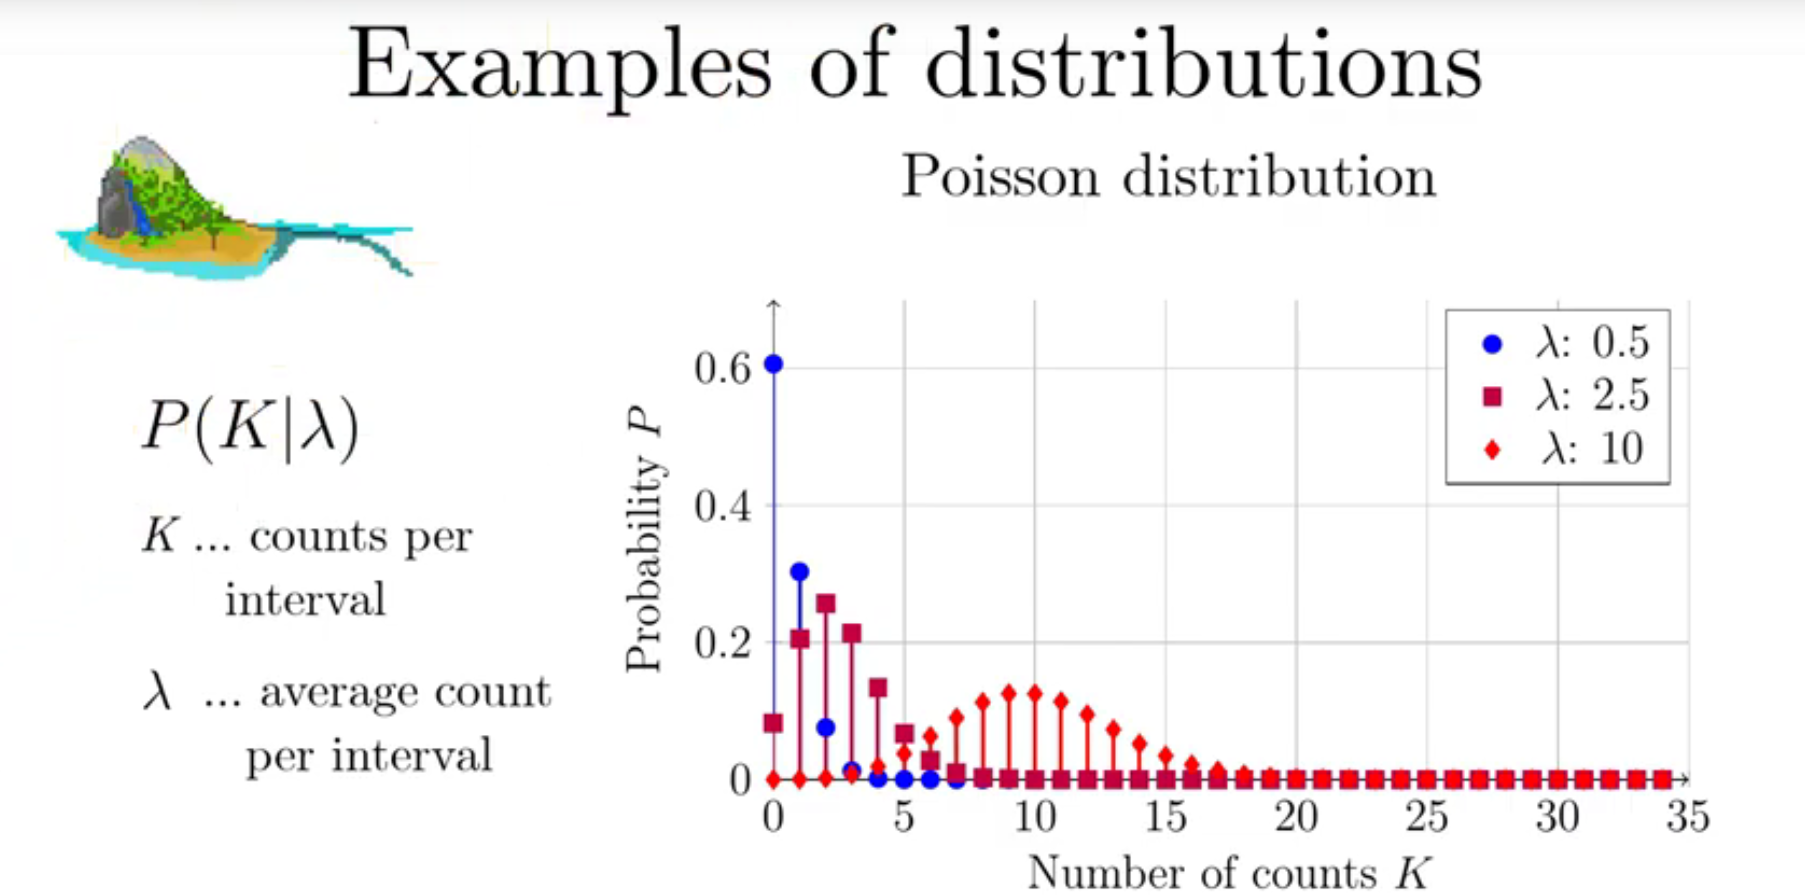
\includegraphics[width=0.75\textwidth]{2_5.png}
\end{figure}

\fbox{\parbox{\linewidth}{\textbf{Question 4.} Complete the sentences with the correct words. ($K$, Poisson, $\lambda$, Binomial, $Q$, $N$, Bernoulli)\\
The ..... distribution describes counting experiments and is characterized by the parameter ...... that describes the average counts per interval.\\
The ..... distribution gives the probability for having ...... successes when performing ........ repeated ....... experiments with a success probability ........ .
}}\\

We will now learn about the characteristic parameters, that will give us important information about the distribution. We will introduce them from two points of view, namely Bernoulli’s view, of \textbf{intrinsic features}, and Venn’s perspective of \textbf{repeated experiments}.
This shall help you to make the link between the two worlds.
Note that the characteristic values, obtained from samples are themselves \textit{random variables}, whereas the characteristic values from the intrinsic probabilities are \textit{fixed numbers}! 
We will use a slightly different notation and wording to distinguish them.\\

The \textbf{mean value}, also called \textbf{expectation value}, describes the location of a distribution.
Based on the intrinsic probabilities the intrinsic mean is a fixed number given by the \textit{weighted sum of the random variable} using the probabilities as weights. One can also calculate the mean of functions of random variables, like $X^2$. We denote the intrinsic mean by angle brackets.
Note that the mean is \textit{linear} - we will study this property a bit later in this unit.\\
\begin{equation*}\boxed{\langle X \rangle := \sum_iP_iX_i \qquad
\langle f(X) \rangle := \sum_iP_if(X_i)}\end{equation*}
From the frequentist perspective, based on a sample of size N, the sample mean is formed by the \textit{arithmetic mean of the sample values}. \\

\begin{equation*}\boxed{\bar{X} := \frac{1}{N}\sum_{\nu=1}^N X_\nu}\end{equation*}

Note that the sample mean varies depending on the sample and describes a random variable. The sample mean will be denoted by an overline. 
Now we turn to the first part of the law of large numbers. It states that \\[0.2cm]
\fbox{\parbox{\linewidth}{\begin{centering}
\textit{The sample mean converges to the intrinsic mean when the sample size N approaches infinity.}\end{centering}}}\\[0.2cm]
\fbox{\parbox{\linewidth}{\textbf{Question 5.} Complete the sentences with the correct words. (angle brackets, overlines)\\
The intrinsic mean is denoted by ...... whereas the sample mean uses ........ .
}}\\

From this relation we can also derive the frequentist definition of probabilities, namely as \textit{relative frequencies in the limit of infinitely large sample size.}\\
\begin{equation*}\boxed{\langle X \rangle = \sum_i \lim_{N\rightarrow \infty} \frac{n_i(X)}{N}X_i}\end{equation*}


Another parameter characterizing the location of a distribution is the \textbf{median}. It is the value of the random variable or the ordered sample set that \textit{splits them into two halfs}, each containing at least 50 percent of the probability masses or number of elements.
Let us illustrate the intrinsic median for the golden nautilus wheel. We need to add up the probabilities in the order of the random variables and stop when we reach or exceed the 50 percent mark for the first time. We see 11+17 is still below the 50 percent threshold but 11+17+28 exceeds it and so the third value of $X$, namely four pennies, is the median.
\begin{figure}[H]
	\centering
	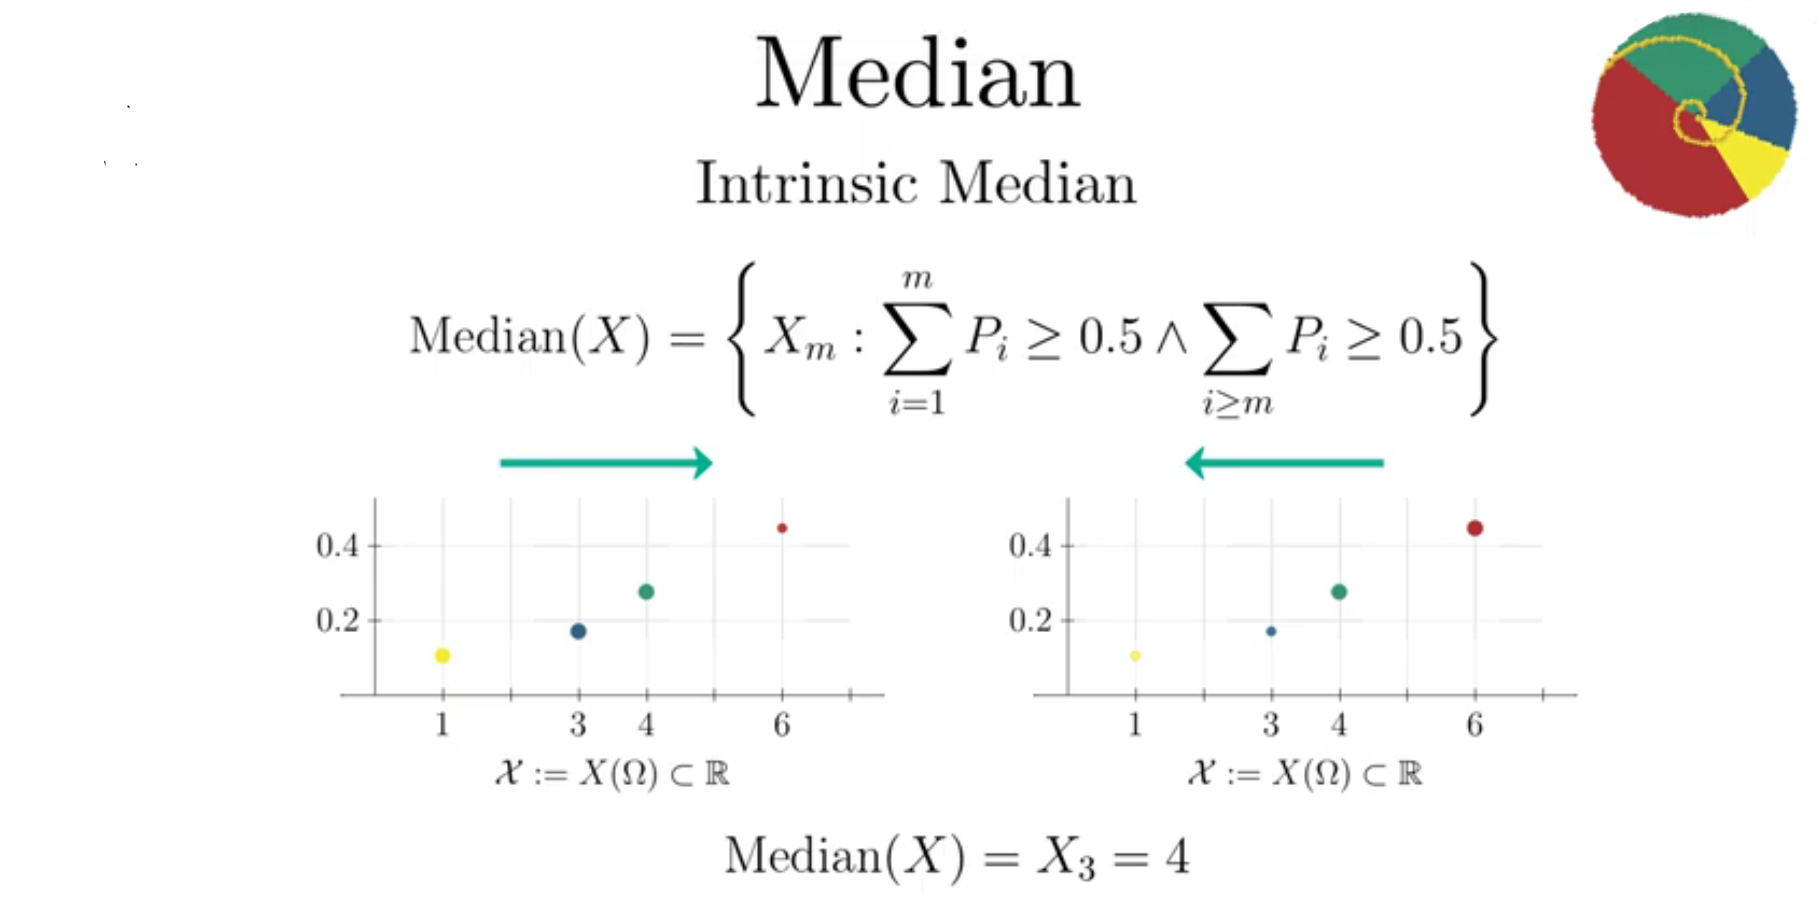
\includegraphics[width=0.75\textwidth]{2_6.png}
\end{figure}
In the precise definition we also have to \textit{sum up the probabilities from right to left}. For the Nautilus wheel we obtain 45+28, which is greater than 50; so the median is again the third value of $X$. The median is not unique if the cumulative probability reaches precisely 50 percent.
For the sample median, one has to \textit{order the sample first and then take the central value}. If the sample size is even, one takes either both central values or the average of both, which in our example is four pennies.
In contrast to the mean, the median is \textit{resilient against outliers}. A single erroneous measurement can severely distort the sample mean, while the sample median remains unchanged.\\
\begin{figure}[H]
	\centering
	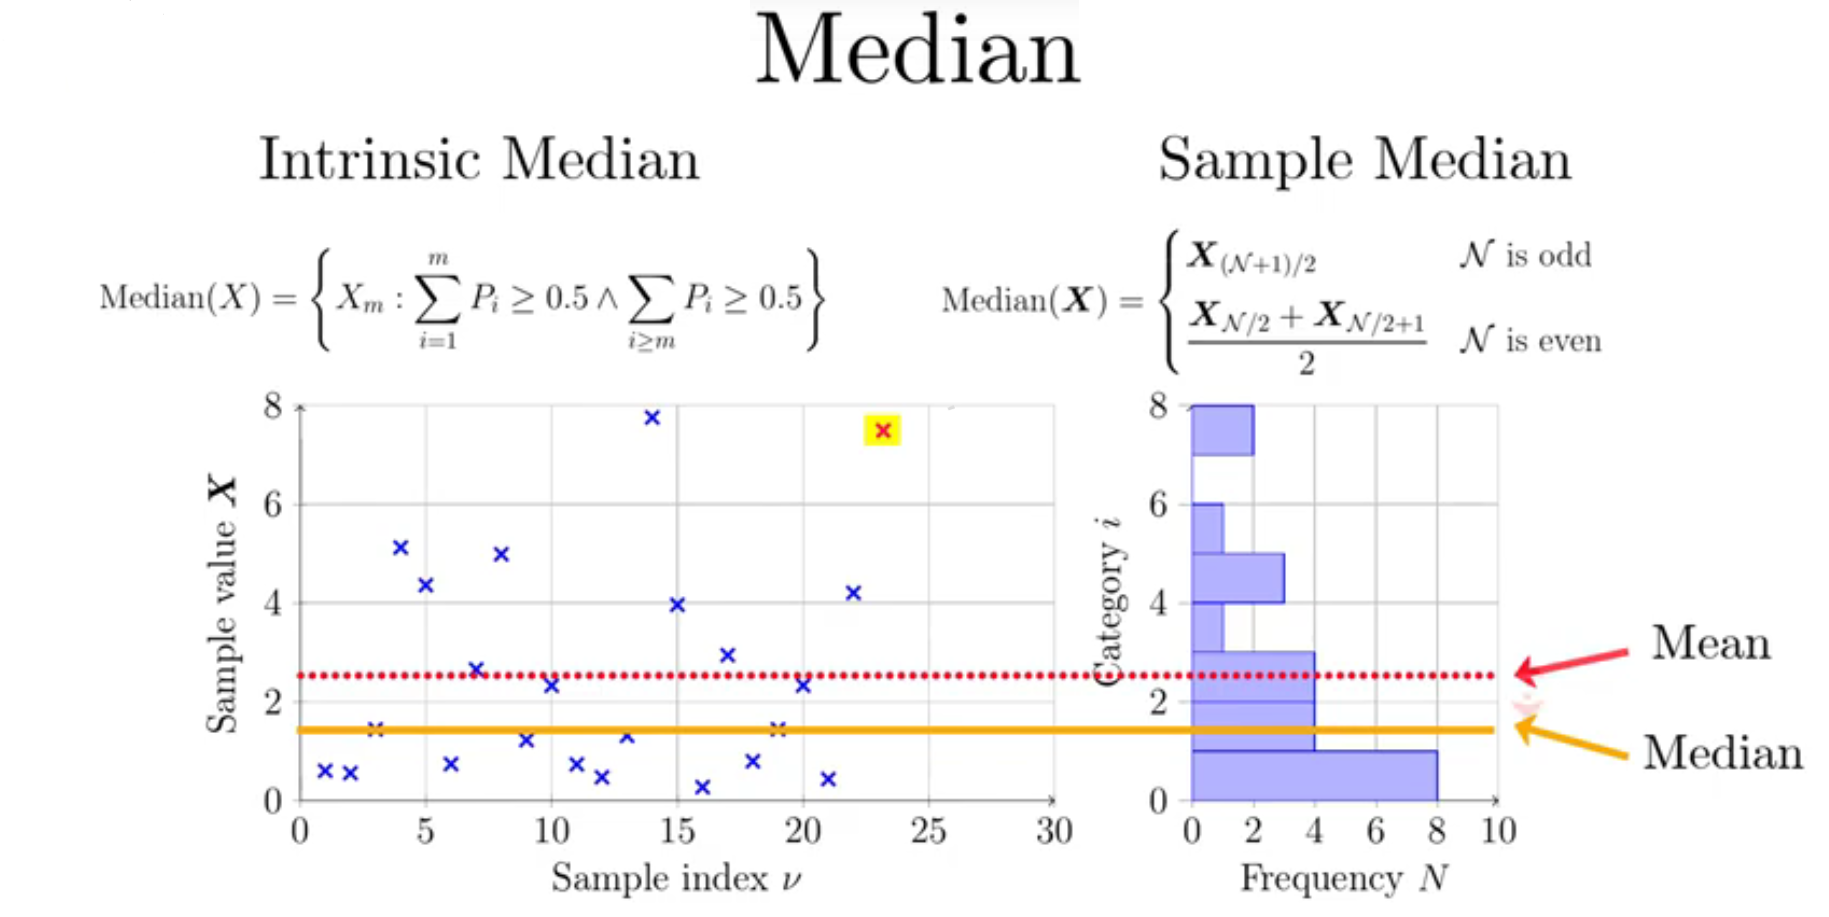
\includegraphics[width=0.75\textwidth]{2_7.png}
\end{figure}
\fbox{\parbox{\linewidth}{\textbf{Question 6.} Which statements are true?\\
a) The sample median can be not-unique if the sample size is even.\\
b) The intrinsic median is not unique if the cummulative probabilities add up to exactly 50\%.\\
c) The intrinsic median can be not-unique if the sample size is odd.\\
d) The mean value is resilient against outliers whereas the median can vary strongly.
}}\\

Besides the location of a distribution the width is also of great importance. It is characterized by the \textbf{variance}, which is the \textit{mean squared deviation of the random variable from its mean}.\\

\begin{equation*}\boxed{\text{Var}(X):=\sum_iP_i(X_i-\langle X \rangle)^2}\end{equation*}

This definition may fall from the sky, but we will discuss fascinating properties of the variance that makes it so powerful.
We see from the definition that the variance has squared units. In order to characterize the width of a distribution we therefore use the \textit{square root} of the variance, which is called \textbf{standard deviation}, and which is denoted by $\sigma$. 
The variance therefore is often labeled with $\sigma^2$. Note that not all values of the distribution have to lie inside the so-called \textbf{1-sigma interval} given by the mean value plus or minus the standard deviation.
Let us now consider the frequentist approach. Given a sample of size $N$ we can pursue the very same strategy and characterize the width of the sample by the mean squared deviation.\\

\begin{equation*}\boxed{\text{Var}(X)=\frac 1N\sum_{\nu = 1}^N(X_\nu-\bar{X})^2}\end{equation*}


The question is: \textit{how does the "sample variance" relate to the true variance?}
There are two things to take into account: 
First, we assume that the individual samples are \textbf{uncorrelated}, meaning that the repeated experiments do not influence each other. For a counter example just think of a random wheel that is pushed so weakly that it barely moves, then you get correlated samples, in which in most cases successive elements are identical.
The second point to be accounted for is, that we actually \textit{don't know the true mean}, but only an estimate given by the sample mean.
Therefore, the \textbf{unbiased sample variance} that estimates the true variance is given by the \textit{sum of the squared deviations from the sample mean divided by $N - 1$}.\\
\begin{equation*}\boxed{\text{Var}(X)=\frac{1}{N-1}\sum_{\nu = 1}^N(X_\nu-\bar{X})^2}\end{equation*}
The meaning of the notion ``unbiased'' will be discussed in a later unit.
The $-1$ in the prefactor can be understood qualitatively as we have used the sample already to compute the sample mean. By doing so, the number of independent deviations ($x_i$ – sample mean) is reduced by one.\\

\fbox{\parbox{\linewidth}{\textbf{Question 7.} Which statements are true?\\
a) The sample variance is biased since the mean value is approxiated with the very same sample set.\\
b)The sample variance converges to the intrinsic variance for large sample size due to the law of large numbers.\\
c) The intrinsic variance can be approximated by the sample variance using the correction factor $N$/$(N-1)$.\\
d) The variance is given in the squared units of the random variable.
}}\\

By now we have learned the two most important characteristics of probability distributions, namely mean and variance.
To deepen our understanding, let's now look at how to use these quantities.
The \textit{weighted average of the k-th power of a random variable }$X$, where the weights are given by the probabilities is a recurring structure and it is named: the \textbf{$k$-th moment} and is denoted by $m_k$.
The $k$-th moment is equivalent to mean of $X^k$.
We can now readily identify the mean as the first moment. 
But what is the 0-th moment? It is the sum of all probabilities and therefore always one.
Finally, the second moment can be calculated directly by substituting $X^2$ into the expression for the mean.\\
\begin{figure}[H]
	\centering
	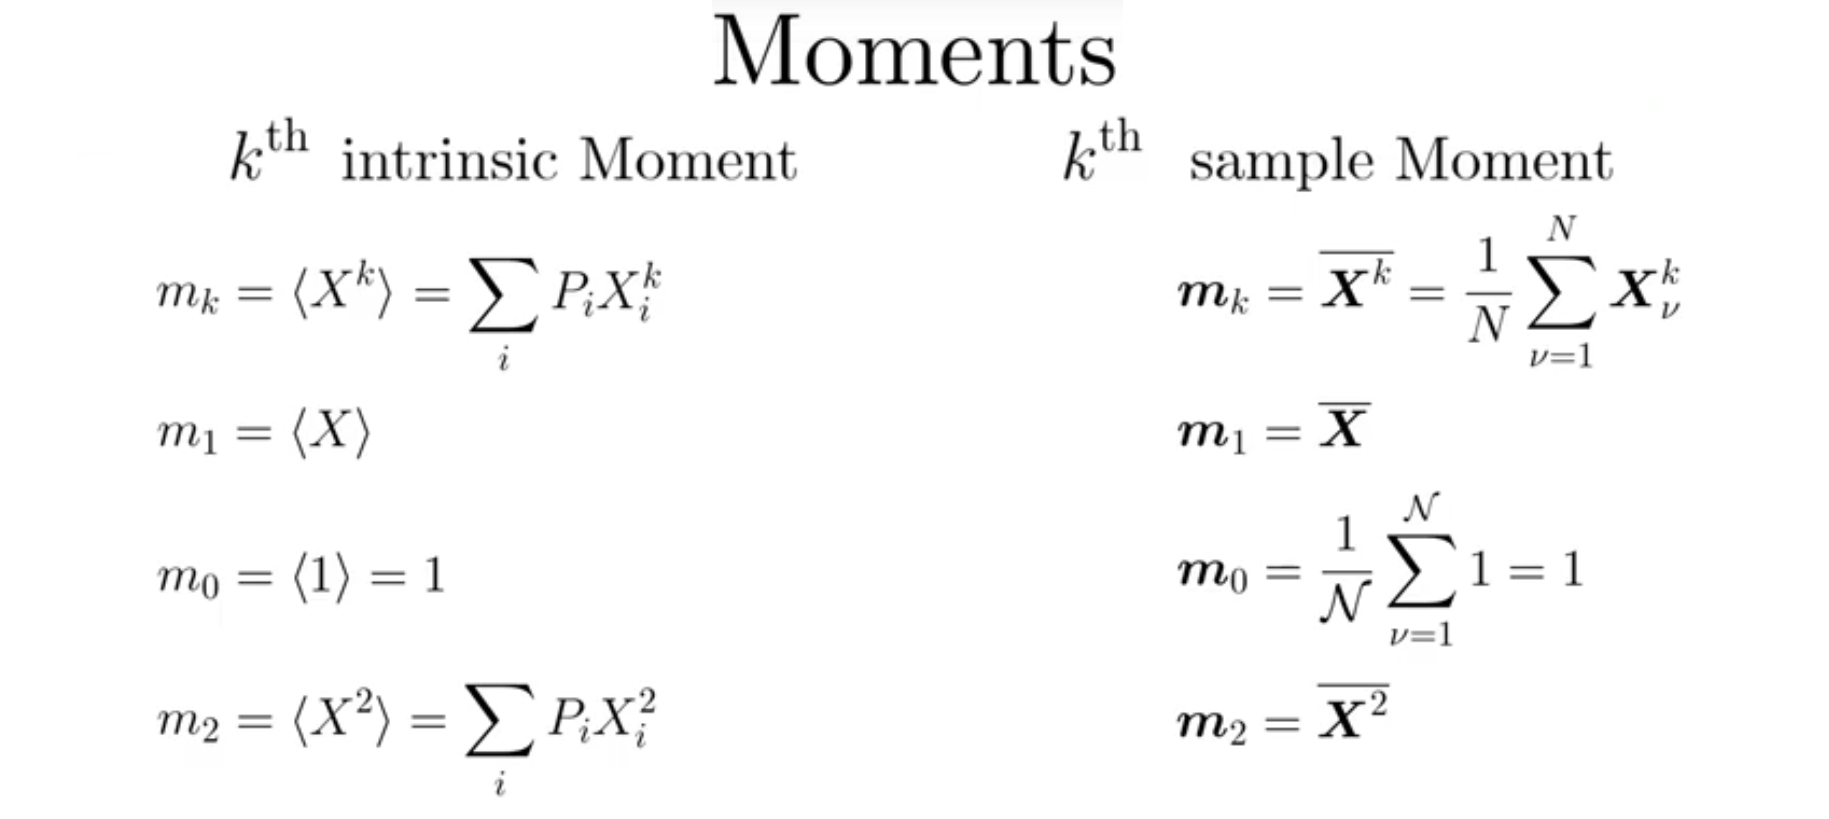
\includegraphics[width=0.75\textwidth]{2_8.png}
\end{figure}

\fbox{\parbox{\linewidth}{\textbf{Question 8.} Calculate the requested values.\\
The second moment of the sample $X=[2321234528]$ is equal to ...... .\\
The second moment of the probability distribution of a dice is ....... .
}}\\

We now practice how we can use the moments to derive a useful relation for the variance.
The variance is given as the mean of the squared deviations from the intrinsic mean – which is also called the \textbf{second central moment}.
Expanding the squared deviations according to the simple binomial theorem results in a sum of three terms.  Due to the linearity, the mean of a sum is the sum of the means. 
We use the fact that already averaged quantities such as the mean are scalar factors that can be drawn out of the angle brackets.
\begin{figure}[H]
	\centering
	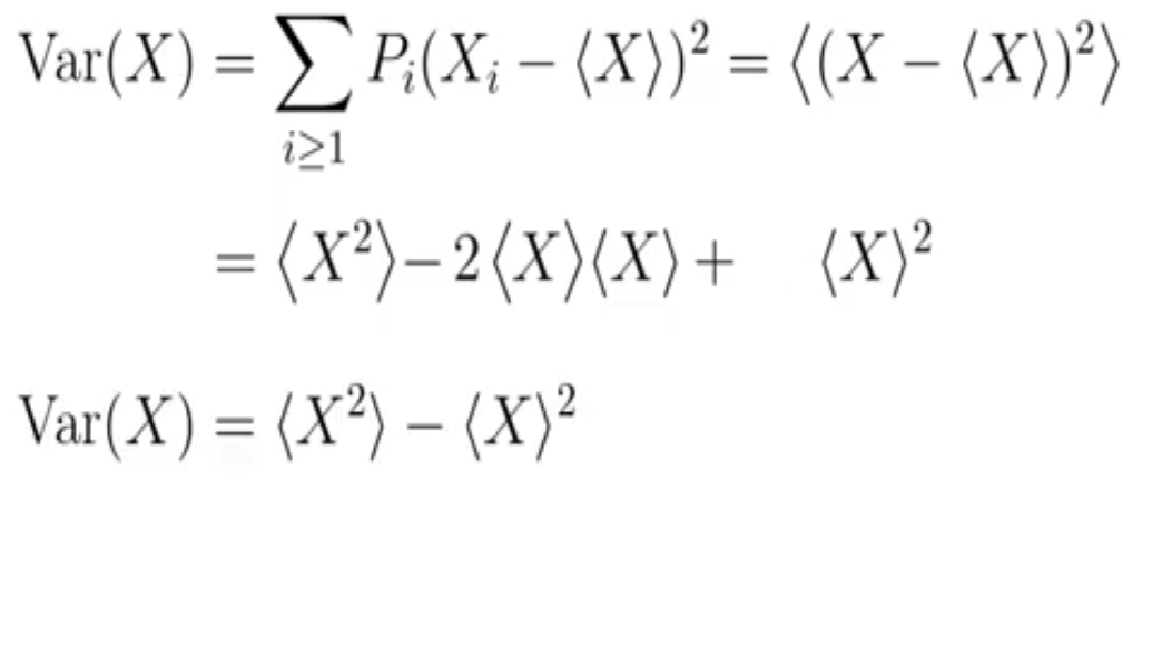
\includegraphics[width=0.75\textwidth]{2_9.png}
\end{figure}
Finally, we obtain the elegant relationship that the variance is the difference between the second moment and the squared first moment.
Similarly, it is straight forward to compute the $k$-th moment based on a sample.
By the same proof we also obtain the useful relation that the sample variance is given by the second sample moment minus the first moment squared.\\

\begin{equation*}\boxed{\text{Var}(X) = \langle X^2 \rangle \qquad \text{Var}(X) = \bar{X^2} - \bar{X}^2}\end{equation*}

\fbox{\parbox{\linewidth}{\textbf{Question 9.} Calculate the requested value.\\
Knowing that the mean value of a probability distribution is $\langle X \rangle = 4$ and the second moment is $\langle X^2\rangle = 25$, the standard deviation is given by StD($X$)= .......... .
}}\\

How can we apply what we learned to help Captain Bayes to answer the questions concerning the wages and the free-days-ratio, both based on the outcome of the golden spiral experiment?
The first question can readily be answered either by using the intrinsic probabilities for the four sectors of the golden spiral, which is Bernoulli’s probabilistic approach or by the statistical description favored by Captain Venn.
Bernoulli computes the mean of the distribution that uses pennies as random variables, which results in approximately 4.4 pennies a day.
The scatter of the wages is given by the standard deviation $\sigma$, which in the present example is 1.66 pennies.
A rule of thumb for most distributions is that you can find about \textit{two-thirds of all outcomes within the 1-$\sigma$ interval}. For the 2-$\sigma$ interval it's roughly 95 \% and the 3-$\sigma$ interval covers almost 99 \% of all cases.
\begin{figure}[H]
	\centering
	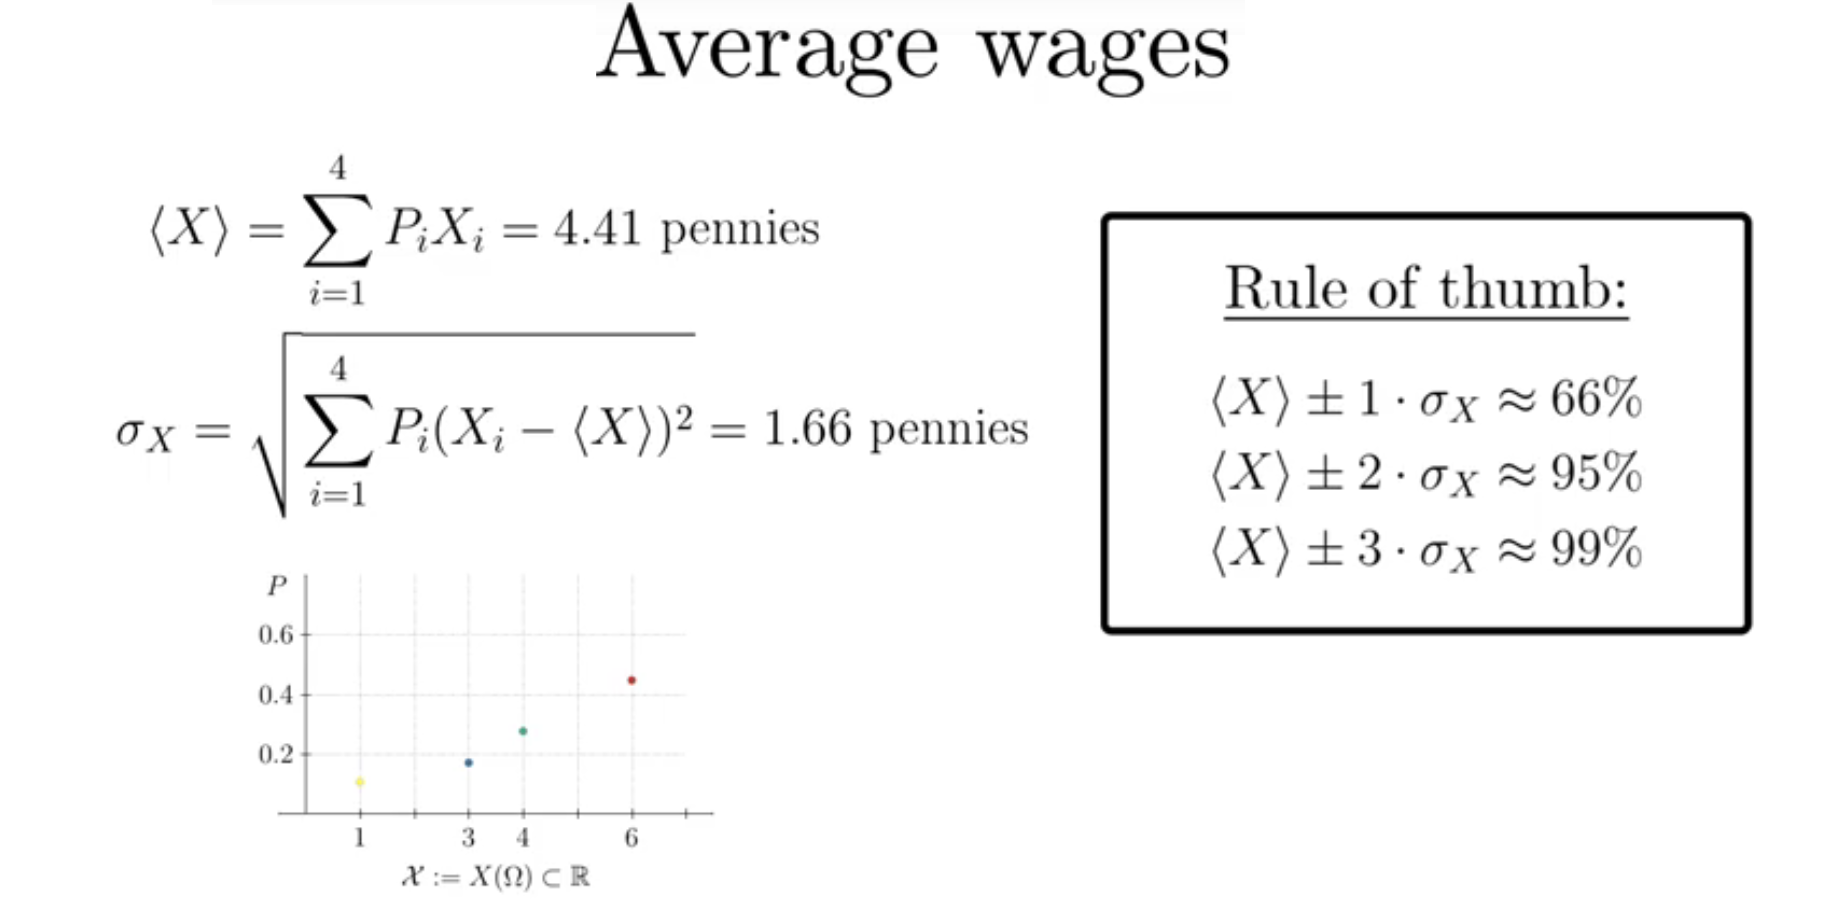
\includegraphics[width=0.75\textwidth]{2_10.png}
\end{figure}
Captain Venn, on the other hand, determines the mean wages based on a sample. Clearly, these results differ from sample to sample.
Note that the variation of the sample mean \textit{depends on the sample size N} and it is quantified by the standard deviation of the sample mean, which is also called \textbf{standard error}.
If the underlying probability distribution has a finite variance, then the standard error of a sample of size $N$ is given by the intrinsic standard deviation divided by $\sqrt{N}$.\\%%formel

This brings us to the second part of the law of large numbers, which according to the standard error states that \\

\fbox{\parbox{\linewidth}{\begin{centering}
\textit{With increasing sample size N, the sample mean approaches the intrinsic mean, like $\frac{1}{\sqrt{N}}$.}\end{centering}}}\\
\begin{figure}[H]
	\centering
	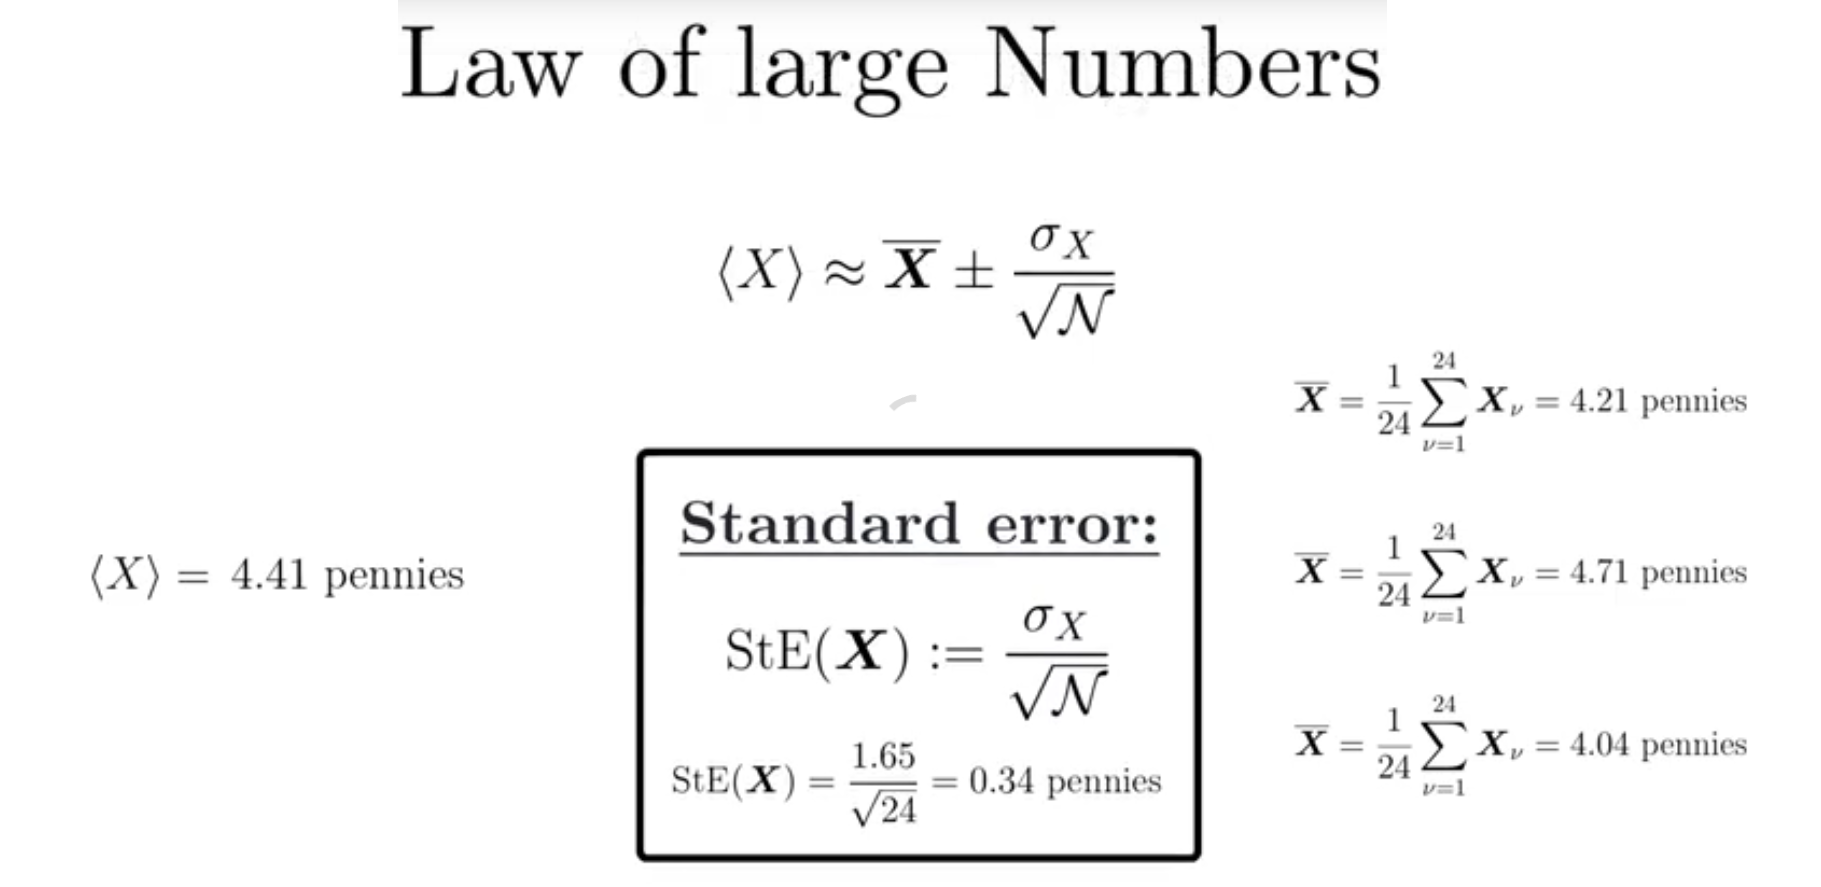
\includegraphics[width=0.75\textwidth]{2_11.png}
\end{figure}

\fbox{\parbox{\linewidth}{\textbf{Question 10.} Practical problem from a production line:\\
Imagine you are monitoring a production line of E-bikes, and take a sample to check the lifetime of the battery.\\
From a sample of 24 bikes, 3 had a broken battery (0 years lifetime), 6 had a weak battery (1 year lifetime) and 15 bikes had the expected lifetime of 2 years. This yields a sample mean value of  $\bar{X}=$...... years.  

What can you say from this sample about the intrinsic mean lifetime $\langle X \rangle$ of the batteries of the E-bikes of that production line?
\textit{Hint: Recall that the sample mean is a random variable $\rightarrow$ Standard error.}
With approximately 66\% the intrinsic mean value lies within the interval of the sample mean value  $\pm$ ....
 years
}}\\

Let's use this insight to answer the second question about the free-days-ratio in a period of $N$ days.
Bernoulli determines the probability of having a day off by using the golden ratio to be 0.106. 
As you can easily see, this is also the average value of the free-days-ratio.
A similar calculation yields for the standard deviation of the free-days-ratio a value of 0.307.
Remember Captain Venn admitted that he could not guarantee a free-days-ratio of at least ten percent for a period of a 1000 days.
To study this point, we repeatedly generate samples of size 1000, compute the sample mean of the free-days-ratio and plot the results as histogram.\begin{figure}[H]
	\centering
	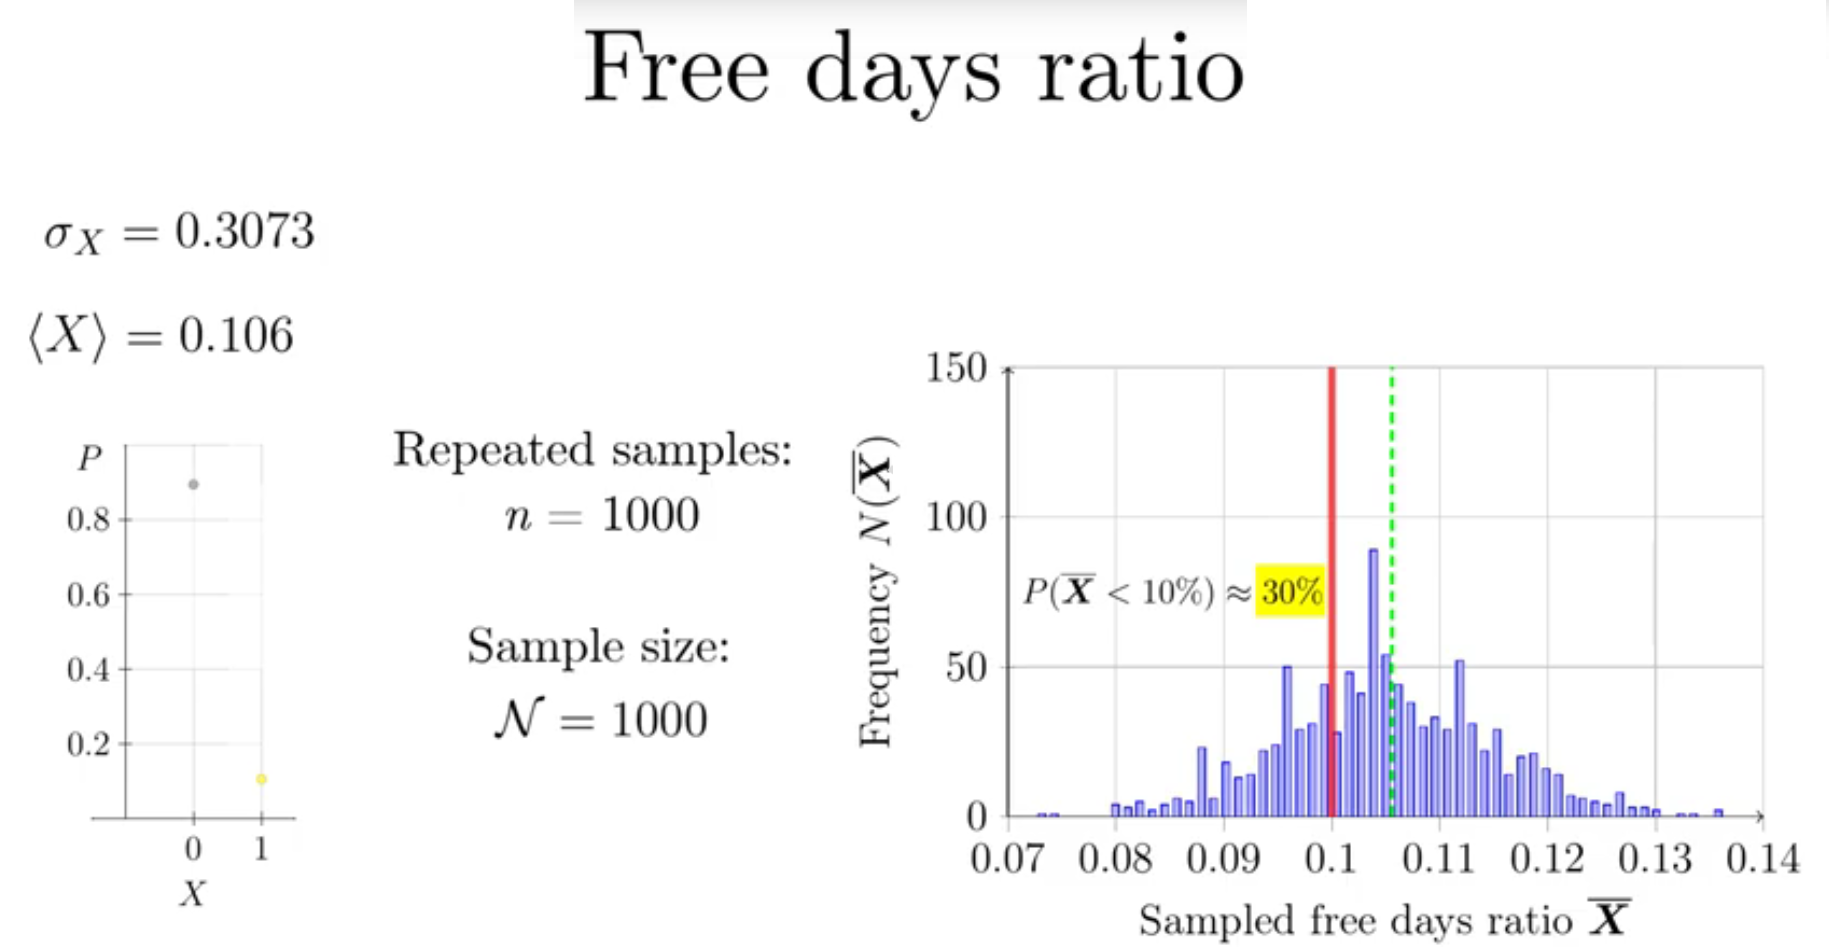
\includegraphics[width=0.75\textwidth]{2_12.png}
\end{figure}
We clearly see that the histogram has a tail that reaches far below the red ten percent line, indicating that there is a high probability to have a free-days ratio less then the required ten percent; corroborating that Captain Venn was right.
Next, we repeat the same analysis for samples of size 10000. Now there is only a very small tail reaching below the red line.
In both cases the standard-error is also included in the histograms indicated by horizontal arrows. Also in this representation we observe that only in the second case the ten percent free-days-ratio can be guaranteed with high probability.\\
\begin{figure}[H]
	\centering
	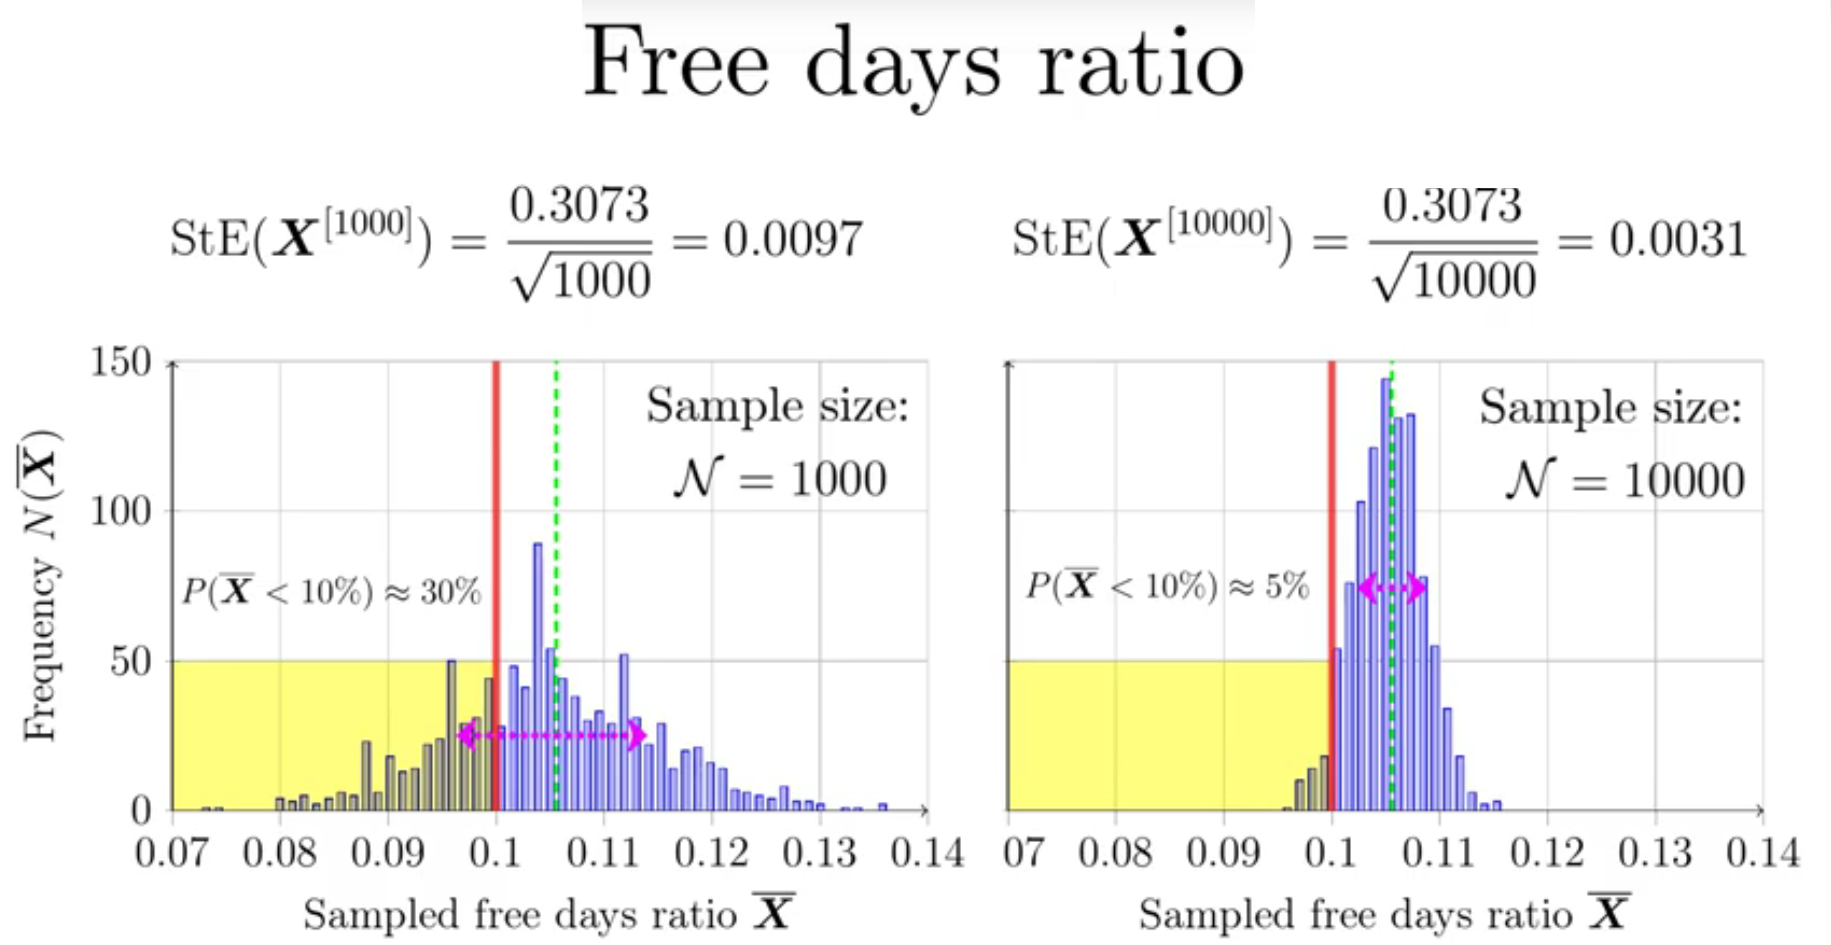
\includegraphics[width=0.75\textwidth]{2_13.png}
\end{figure}
We have reached the end of the second unit. 
Get to know the frequentist approach with the interactive simulation.
Feel free to ask questions in the forum and feel encouraged to test your knowledge in the quiz!


\vspace{2cm}
\begin{minipage}[t]{1\textwidth}
	\raggedleft
	\centering
	
\includegraphics[width = 0.20\textwidth]{CC-BY_icon}
	\vspace{0.2cm}
	
	\centering
	{\large ITPCP, TU Graz} \\
	https://creativecommons.org/licenses/by/4.0/legalcode
\end{minipage}

\end{document}